\documentclass[]{article}

% Imported Packages
%------------------------------------------------------------------------------
\usepackage{amssymb}
\usepackage{amstext}
\usepackage{amsthm}
\usepackage{amsmath}
\usepackage{enumerate}
\usepackage{fancyhdr}
\usepackage[margin=1in]{geometry}
\usepackage{graphicx}
\usepackage{float}
% \usepackage{extarrows}
\usepackage{setspace}
\usepackage{float}
\usepackage{array}
\usepackage{tabularx}
%------------------------------------------------------------------------------

% Header and Footer
%------------------------------------------------------------------------------
\pagestyle{plain}  
\renewcommand\headrulewidth{0.4pt}                                      
\renewcommand\footrulewidth{0.4pt}                                    
%------------------------------------------------------------------------------

% Title Details
%------------------------------------------------------------------------------
\title{Deliverable \#3 Template}
\author{SE 3A04: Software Design II -- Large System Design}
\date{}                               
%------------------------------------------------------------------------------

% Document
%------------------------------------------------------------------------------
\begin{document}

\maketitle	
\noindent{\bf Tutorial Number:} T01\\
{\bf Group Number:} G4 \\
{\bf Group Members:} Lukas Buehlmann, David Olejniczak,Vanessa Lai, Saqib Khan, Suzanne Abdullah


\section*{IMPORTANT NOTES}
\begin{itemize}
	\item You do \underline{NOT} need to provide a text explanation of each diagram; the diagram should speak for itself
	\item Please document any non-standard notations that you may have used
	\begin{itemize}
		\item \emph{Rule of Thumb}: if you feel there is any doubt surrounding the meaning of your notations, document them
	\end{itemize}
	\item Some diagrams may be difficult to fit into one page
	\begin{itemize}
		\item It is OK if the text is small but please ensure that it is readable when printed
		\item If you need to break a diagram onto multiple pages, please adopt a system of doing so and throughly explain how it can be reconnected from one page to the next; if you are unsure about this, please ask me
	\end{itemize}
	\item Please submit the latest version of Deliverable 1 and Deliverable 2 with Deliverable 3
	\begin{itemize}
		\item They do not have to be a freshly printed versions; the latest marked versions are OK
	\end{itemize}
	\item If you do \underline{NOT} have a Division of Labour sheet, your deliverable will \underline{NOT} be marked
\end{itemize}
\newpage

\section{Introduction}
\label{sec:introduction}
% Begin Section

\subsection{Purpose}
\label{sub:purpose}
% Begin SubSection
This document provides further information about the SCHEMAS system architecture, including state chart diagrams, sequence diagrams, and a detailed class diagram. 
\newline \\
This document is intended for internal SCEHMAS stakeholders, including but not limited to project managers, developers, domain experts, and SCEHMAS team members/investors. SCEHMAS Deliverables 1 and 2 should be read prior to, and technical knowledge may be beneficial in better understanding the contents of the document.


% End SubSection

\subsection{System Description}
\label{sub:system_description}
% Begin SubSection
	 This system will monitor real-time sensor data input from across a city to measure environmental changes. The system will be primarily used by city operators who have access to a dashboard which shows recent data aggregated over time as well as environmental alerts. The management of alerts and accounts is done by administrators who have greater permissions than other users. The system will also expose a REST API for public users which only exposes non-sensitive environmental data aggregated by city zone. The system will also have an app for public users to easily view data from the API. All major actions are logged for audit purposes and the system implements rate-limiting to prevent denial-of-service attacks and to maintain high uptime. 
% End SubSection

\subsection{Overview}
\label{sub:overview}
% Begin SubSection
	This document is organized into an introduction followed by sections for various types of charts used to describe the structure and behaviour of the system. Each section will be focused on a different type of diagram. Section 2 contains State Charts for each of the controller classes. Section 3 contains Sequence Diagrams representing each use case of the system. Section 4 contains a detailed Class Diagram for the system. 

% End SubSection

% End Section

\section{State Charts for Controller Classes}
\label{sec:state_charts_for_controller_classes}
% Begin Section

\begin{figure}[H]
    \centering
    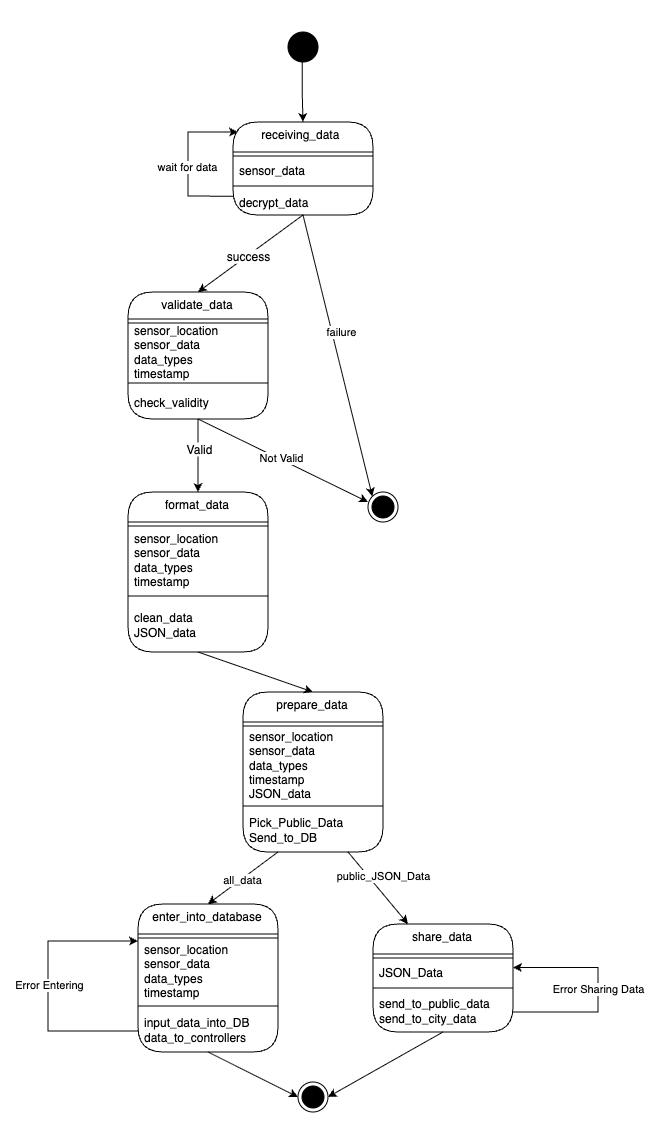
\includegraphics[width=0.75\textwidth]{ImagesD3/StateProcessingofSensorData.png}
    \caption{\textbf{Processing of Sensor Data State Diagram}}
    \label{fig:Processing of Sensor Data State Diagram}
\end{figure}


\begin{figure}[H]
    \centering
    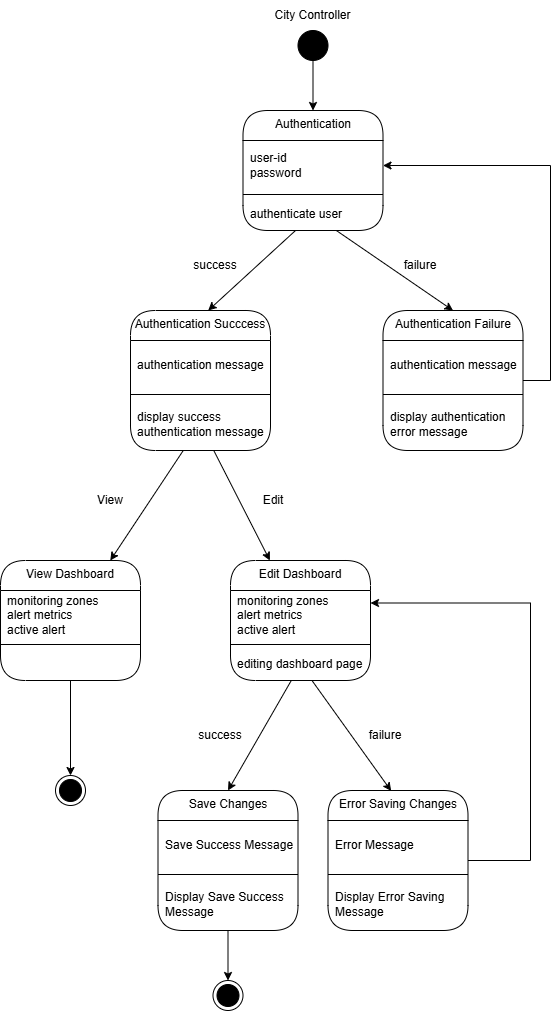
\includegraphics[width=0.75\textwidth]{ImagesD3/State City Controller.png}
    \caption{\textbf{City Controller State Diagram}}
    \label{fig: City Controller State Diagram}
\end{figure}

\begin{figure}[H]
    \centering
    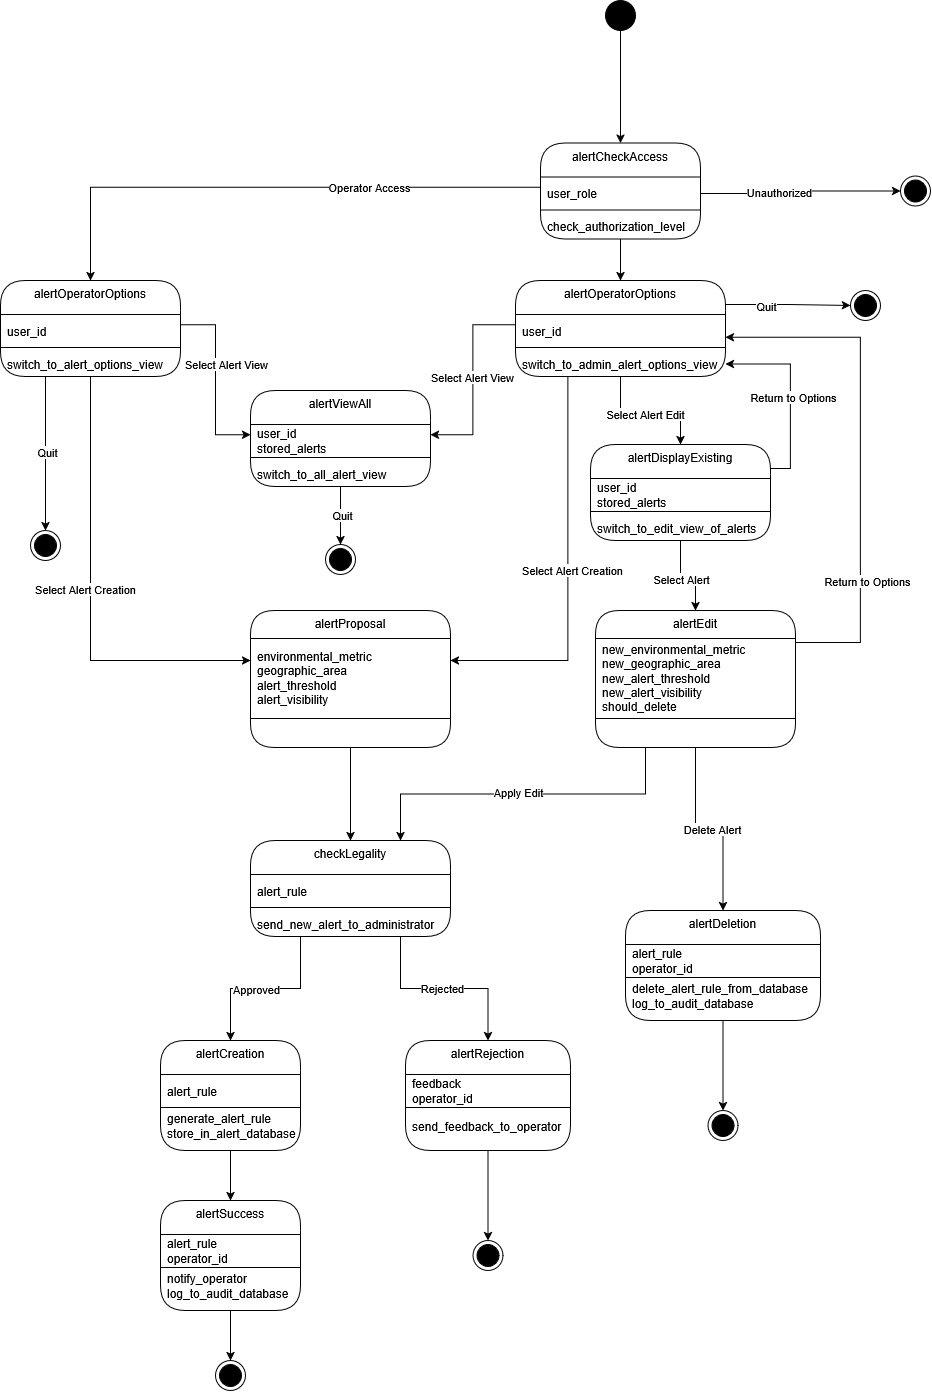
\includegraphics[width=0.75\textwidth]{ImagesD3/State_Alert_Management.png}
    \caption{\textbf{Alert Management State Diagram}}
\end{figure}

\begin{figure}[H]
    \centering
    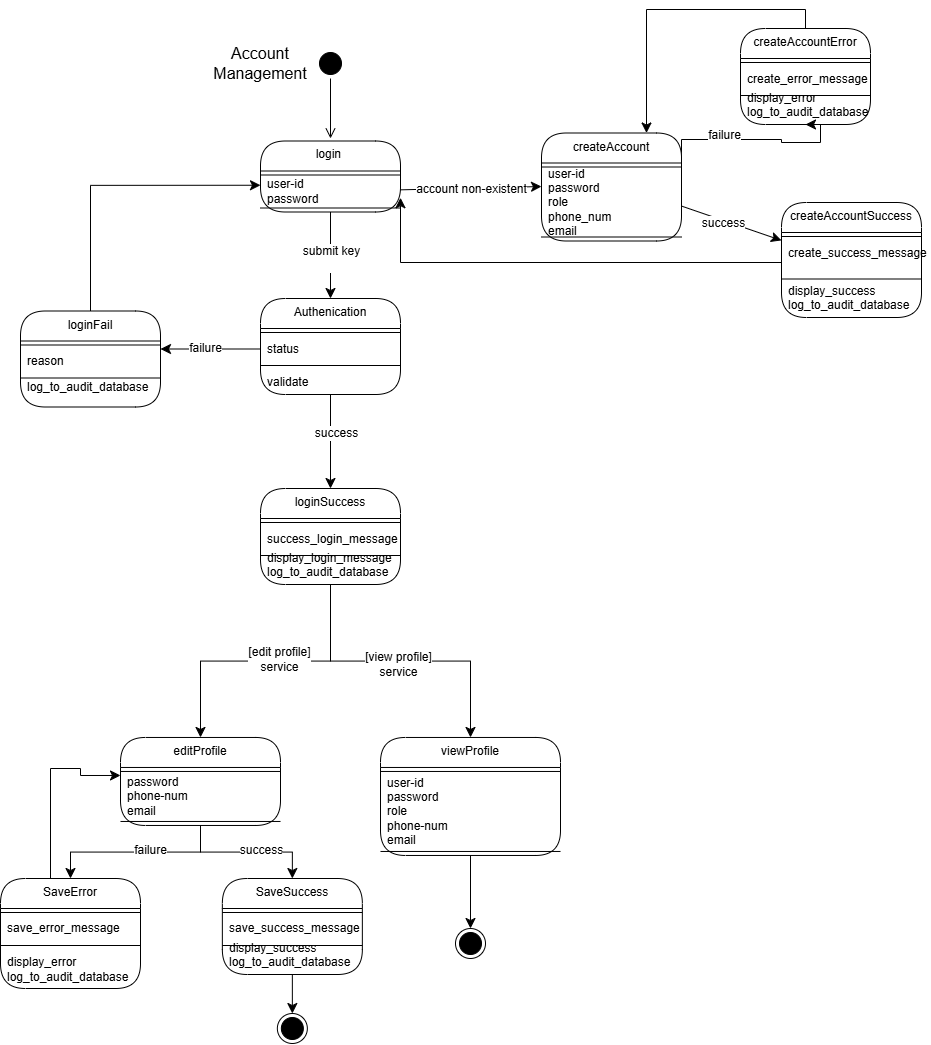
\includegraphics[width=0.75\textwidth]{ImagesD3/State Account Management.png}
    \caption{\textbf{Account Management State Diagram}}
    \label{fig:Account Management State Diagram}
\end{figure}
% End Section

\section{Sequence Diagrams}
\label{sec:sequence_diagrams}
% Begin Section

\begin{figure}[H]
    \centering
    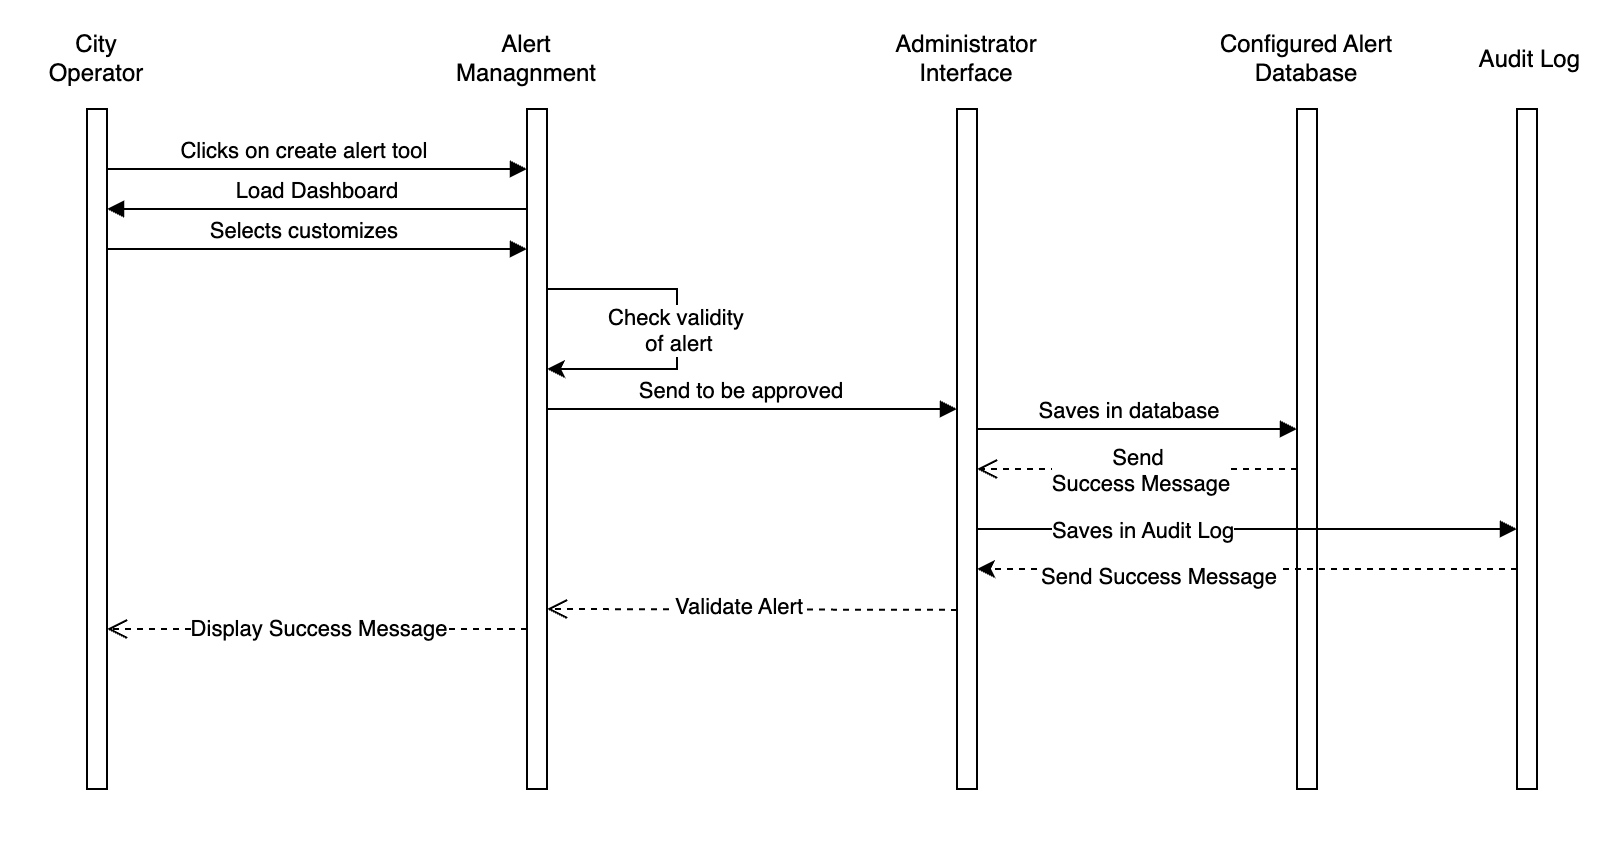
\includegraphics[width=1\linewidth]{ImagesD3/BE1.png}
    \caption{\textbf{Creating an Alert Rule}}
    \label{fig:Creating an Alert Rule}
\end{figure}

\begin{figure}[H]
    \centering
    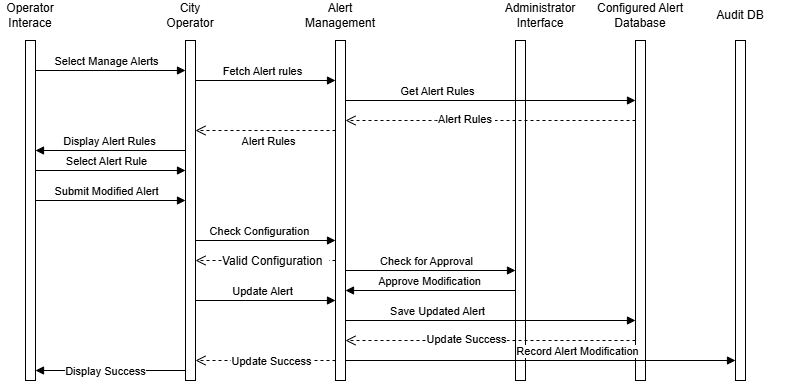
\includegraphics[width=1\linewidth]{ImagesD3/BE2.png}
    \caption{\textbf{Modifying Alert}}
    \label{fig:BE2 Modifying Alert}
\end{figure}

\begin{figure}[H]
    \centering
    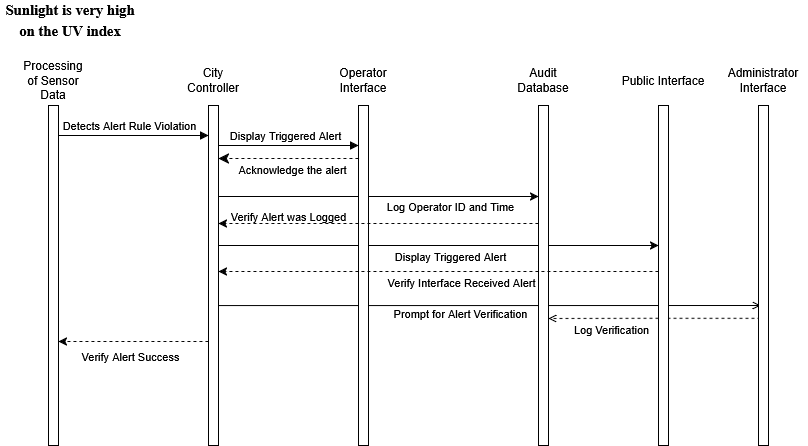
\includegraphics[width=1\linewidth]{ImagesD3/BE3.png}
    \caption{\textbf{Sunlight is very high on the UV index}}
    \label{fig:BE3 Sunlight is very high on the UV index}
\end{figure}

\begin{figure}[H]
\centering
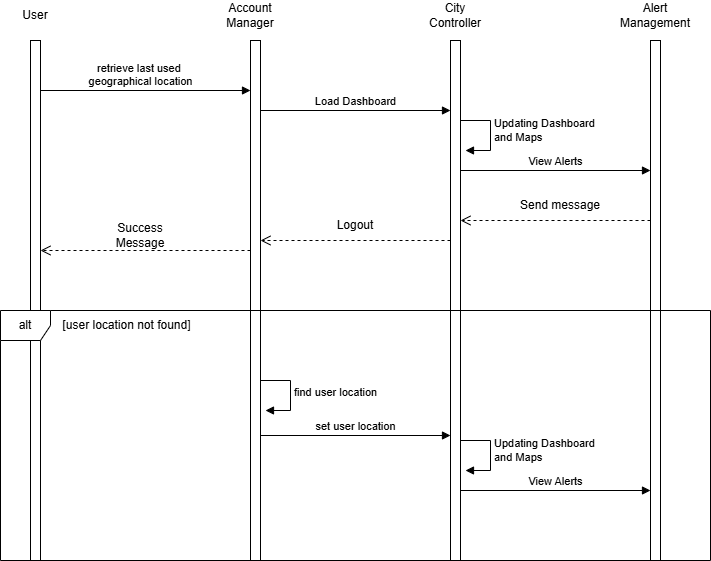
\includegraphics[width=0.75\textwidth]{ImagesD3/BE4 Sequence Diagram.png}
\caption{\textbf{View Dashboard Sequence Diagram}}
\end{figure}


\begin{figure}[H]
    \centering
    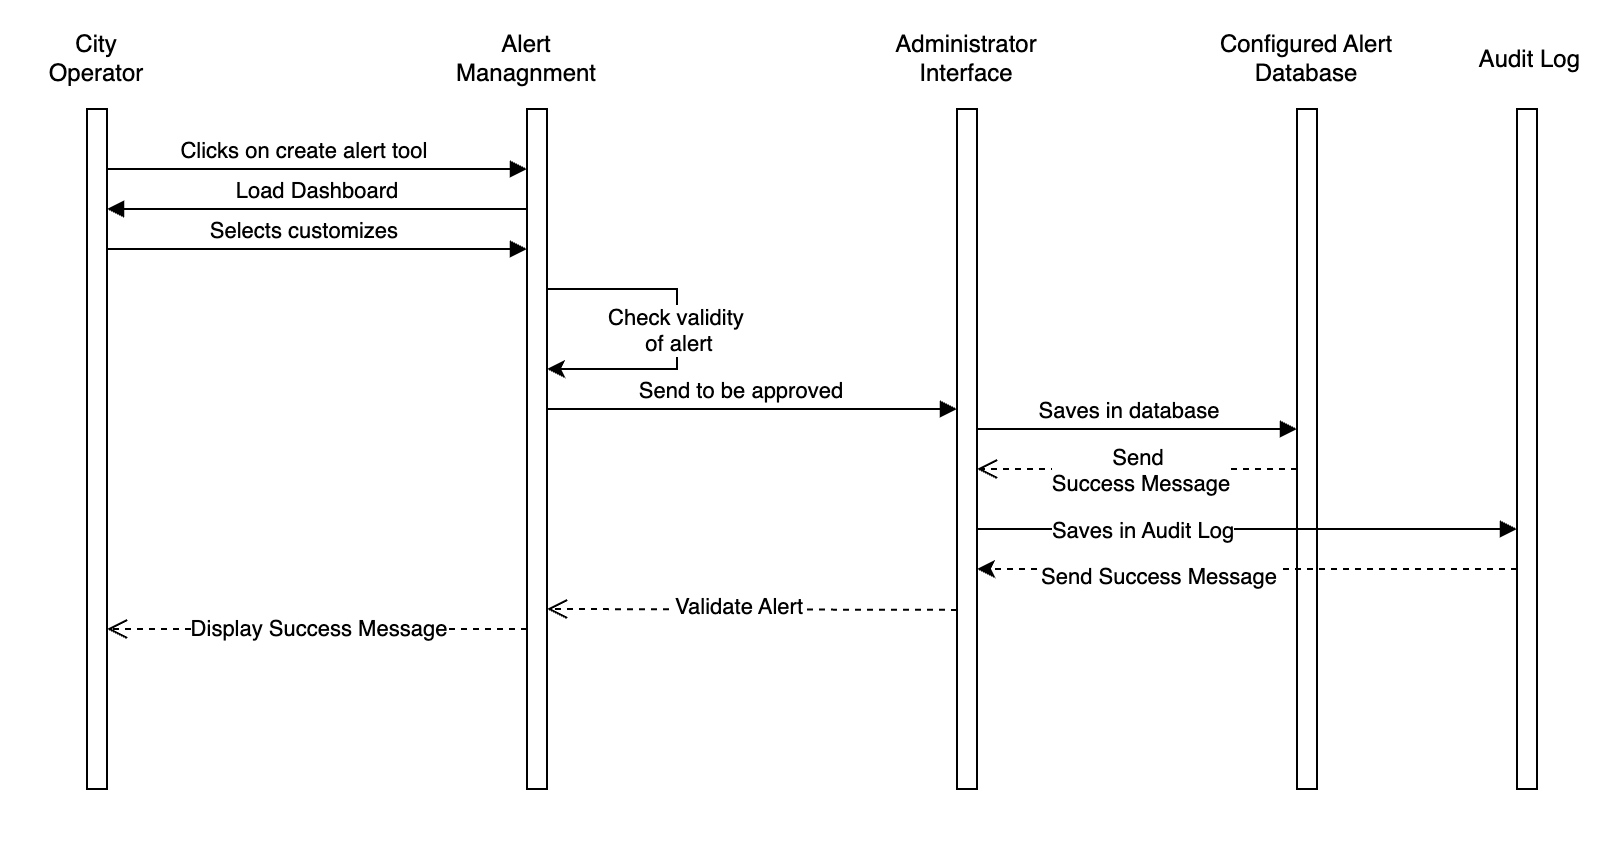
\includegraphics[width=1\linewidth]{ImagesD3/BE5.png}
    \caption{\textbf{Public API Request to Access Data}}
    \label{fig:BE5 Public API Request to Access Data}
\end{figure}

\begin{figure}[H]
    \centering
    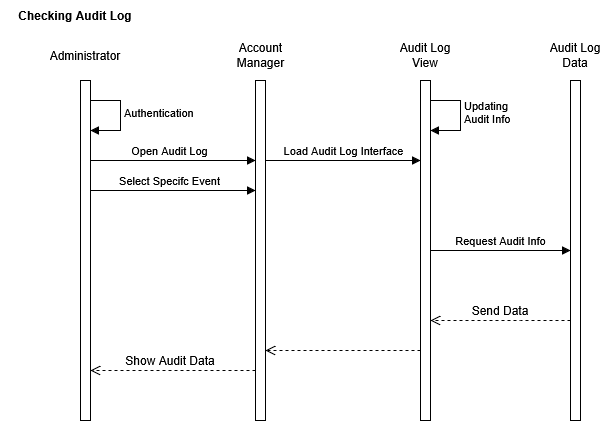
\includegraphics[width=1\linewidth]{ImagesD3/BE6.png}
    \caption{\textbf{Checking Audit Log}}
    \label{fig:BE6 Checking Audit Log}
\end{figure}

\begin{figure}[H]
    \centering
    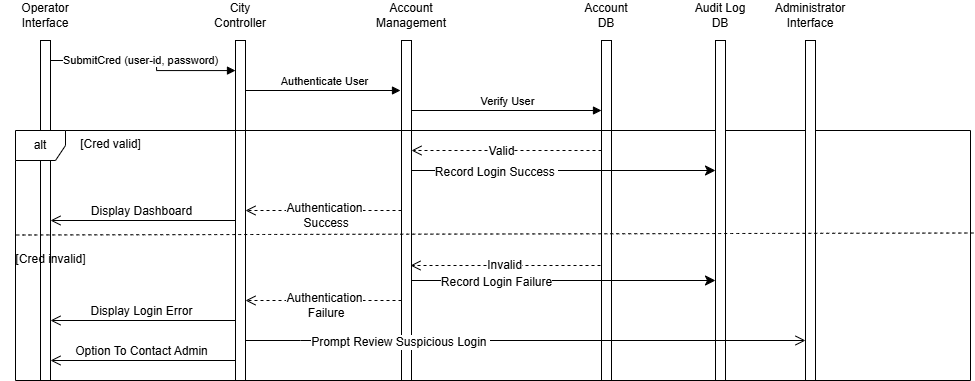
\includegraphics[width=1\linewidth]{ImagesD3/BE7.png}
    \caption{\textbf{User Authentication}}
    \label{fig:User Authentication}
\end{figure}


% End Section

\section{Detailed Class Diagram}
\label{sec:detailed_class_diagram}
% Begin Section

% End Section

\appendix
\section{Division of Labour}
\label{sec:division_of_labour}
% Begin Section
This sheet indicates the contributions of each team member and is signed by all team members. \newline

\noindent
Olejniczak, David
\begin{itemize}
\item Section 2, Created the Processing of Sensor Data State Diagram
\item Section 3, Created the sequence diagram for BE1 
\item Section 3, Created the sequence diagram for BE5 
\item Section 4, Helped creating the Class Diagram
\item Helped write format the LaTeX document

\end{itemize}

\includegraphics[width=0.3\textwidth]{images/David}

\noindent
Khan, Saqib
\begin{itemize}
\item Section 2, State chart for controller class: Account Management
\item Section 3, Sequence Diagram for BE2 - Modifying Alert
\item Section 3, Sequence Diagram for BE7 - User Authentication
\item Contributed to Section 4: Account-related Class Diagram
\item Revised D1 BE2
\item Helped write and format LaTeX document
\end{itemize}

\includegraphics[width=0.3\textwidth]{images/Saqib}

\noindent
Lai, Vanessa
\begin{itemize}
\item Section 2, Created the City Controller State Diagram
\item Section 3, Created the sequence diagram for BE4  View Dashboard 
\item Section 4, Helped creating the Class Diagram (Alert Management Related)
\item Helped write format the LaTeX document
\end{itemize}

\includegraphics[width=0.3\textwidth]{images/Vanessa.png}

\noindent
Abdullah, Suzanne
\begin{itemize}
\item Section 2, State chart for controller class: Public Controller
\item Section 3, Created the sequence diagram for BE6 checking audit log
\item Section 4, Helped creating the Class Diagram (Audit Log classes)
\item Helped write format the LaTeX document
\end{itemize}

\includegraphics[width=0.3\textwidth]{images/Suzanne}


% End Section




\end{document}
%------------------------------------------------------------------------------
